\bigskip

\item The graph below represents which function? 

% \resizebox{3in}{!}{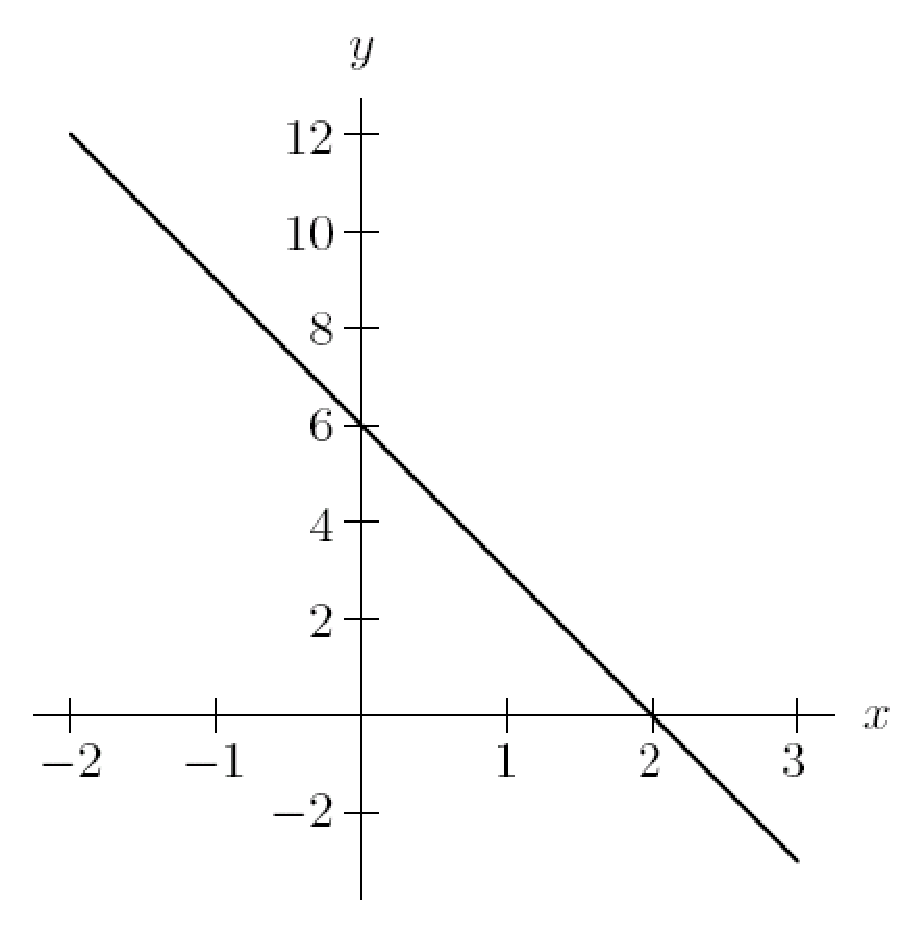
\includegraphics{SVC.01.01.090.ps}}
    \begin{minipage}{0.5\columnwidth}
        \begin{enumerate}
            \item $y = 6x + 6$
            \item $y = -3x + 6$
            \item $y = -3x + 2$
            \item $y = -x+ 6$
            \item $y = 6x -2$
            \item $y = x -2$
        \end{enumerate}
    \end{minipage}
    \begin{minipage}{0.5\columnwidth}
        \begin{tikzpicture}
            \begin{axis}[axis lines=center, xlabel={$x$}, ylabel={$y$}, xmin=-2, xmax=3,
                ymin=-3, ymax=13, ytick={-2,2,4,6,8,10,12}]
                \addplot[color=blue, very thick] {6-3*x};
            \end{axis}
        \end{tikzpicture}
    \end{minipage}


% ConcepTests - to accompany Calculus 4th Edition, Hughes-Hallet et al. John Wiley \& Sons.
